\Chapter{Название главы 1}
\section{раздел1}
\lipsum[1-3]

dgdfg dfgfd gf dfg dfg dfg fdg \ref{fig:structure2}  \ref{tab:table1}

hi there !
привет, там!
правет   \cite{nik} \cite{nik} \cite{nik} \cite{nik}  \cite{test}  \cite{ivanov}  \cite{test}
\cite{kr_privet}
\cite{abadi}
\cite{abadi2}
"<there">

абзац1 абзац1 абзац1 абзац1 абзац1 абзац1 абзац1 абзац1 абзац1 абзац1 абзац1 
$E=mc^{2}$ $A=\frac{E}{mc^{4}}$
абзац1 абзац1  абзац1  абзац1  абзац1  абзац1  абзац1  абзац1  абзац1  абзац1  абзац1  абзац1  абзац1  абзац1  абзац1  абзац1  абзац1  абзац1  абзац1 

$E=mc^{2}$

\[E=mc^{2}\]

\begin{equation} 
 f(x)=(x+a)(x+b),
\end{equation}
\begin{equation} 
 f(x)=(x+a)(x+b),
\end{equation}

\[
 \lim_{x\to 0}{\frac{e^x-1}{2x}}
 \overset{\left[\frac{0}{0}\right]}{\underset{\mathrm{H}}{=}}
 \lim_{x\to 0}{\frac{e^x}{2}}={\frac{1}{2}}
\]

\begin{equation} 
 f(x)=(x+a)(x+b)
\end{equation}

\[A=\frac{E}{m\frac{1}{c^{4}}},\]

\[E=mc^{2},\]

\[E=mc^{2}\]

абзац2 абзац2 абзац2 абзац2 абзац2 абзац2 абзац2 абзац2 абзац2 абзац2 абзац2 абзац2 абзац2 абзац2 абзац2 абзац2 абзац2 абзац2 абзац2 


\begin{figure}
\centering
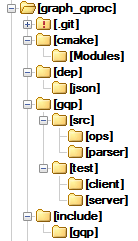
\includegraphics[scale=1]{structure}
\caption{Дерево файлов проекта Дерево файлов проекта Дерево файлов проекта Дерево файлов проекта Дерево файлов проекта }
\label{fig:structure}
\end{figure}

\begin{figure}
\centering
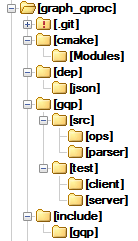
\includegraphics[scale=1]{structure}
\caption{Дерево файлов проекта}
\label{fig:structure1}
\end{figure}

\begin{figure}
\centering
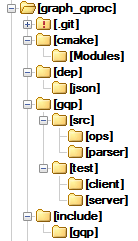
\includegraphics[scale=1]{structure}
\caption{Дерево файлов проекта}
\label{fig:structure2}
\end{figure}


\begin{table}
\caption{Дерево файлов проекта}
\label{tab:table1}
\centering
\begin{tabular}{|c|c|}
\hline
a & A\\
\hline
b & b\\
\hline
\end{tabular}
\end{table}

\begin{table}
\caption{Дерево файлов проекта Дерево файлов проекта Дерево файлов проекта Дерево файлов проекта Дерево файлов проекта Дерево файлов проекта Дерево файлов проекта Дерево файлов проекта }
\label{tab:table2}
\centering
\begin{tabular}{|c|c|}
\hline
a & A\\
\hline
b & b\\
\hline
\end{tabular}
\end{table}

\begin{table}
\caption{Дерево файлов проекта}
\label{tab:table3}
\centering
\begin{tabular}{|c|c|}
\hline
a & A\\
\hline
b & b\\
\hline
\end{tabular}
\end{table}

\lipsum[1]
\section{раздел2}
\section{раздел3}